\documentclass{article}

\usepackage{graphicx}
\usepackage{tikz}
\usepackage{tikzsymbols}
\usetikzlibrary{calc,patterns,shapes.geometric}
\pagestyle{empty}
\usepackage[margin=0pt]{geometry}
\geometry{papersize={14in,12in}}

\def\centerarc[#1](#2)(#3:#4:#5){\draw[#1] ($(#2)+({#5*cos(#3)},{#5*sin(#3)})$) arc (#3:#4:#5);}

\begin{document}
	\begin{figure}
		\centering
		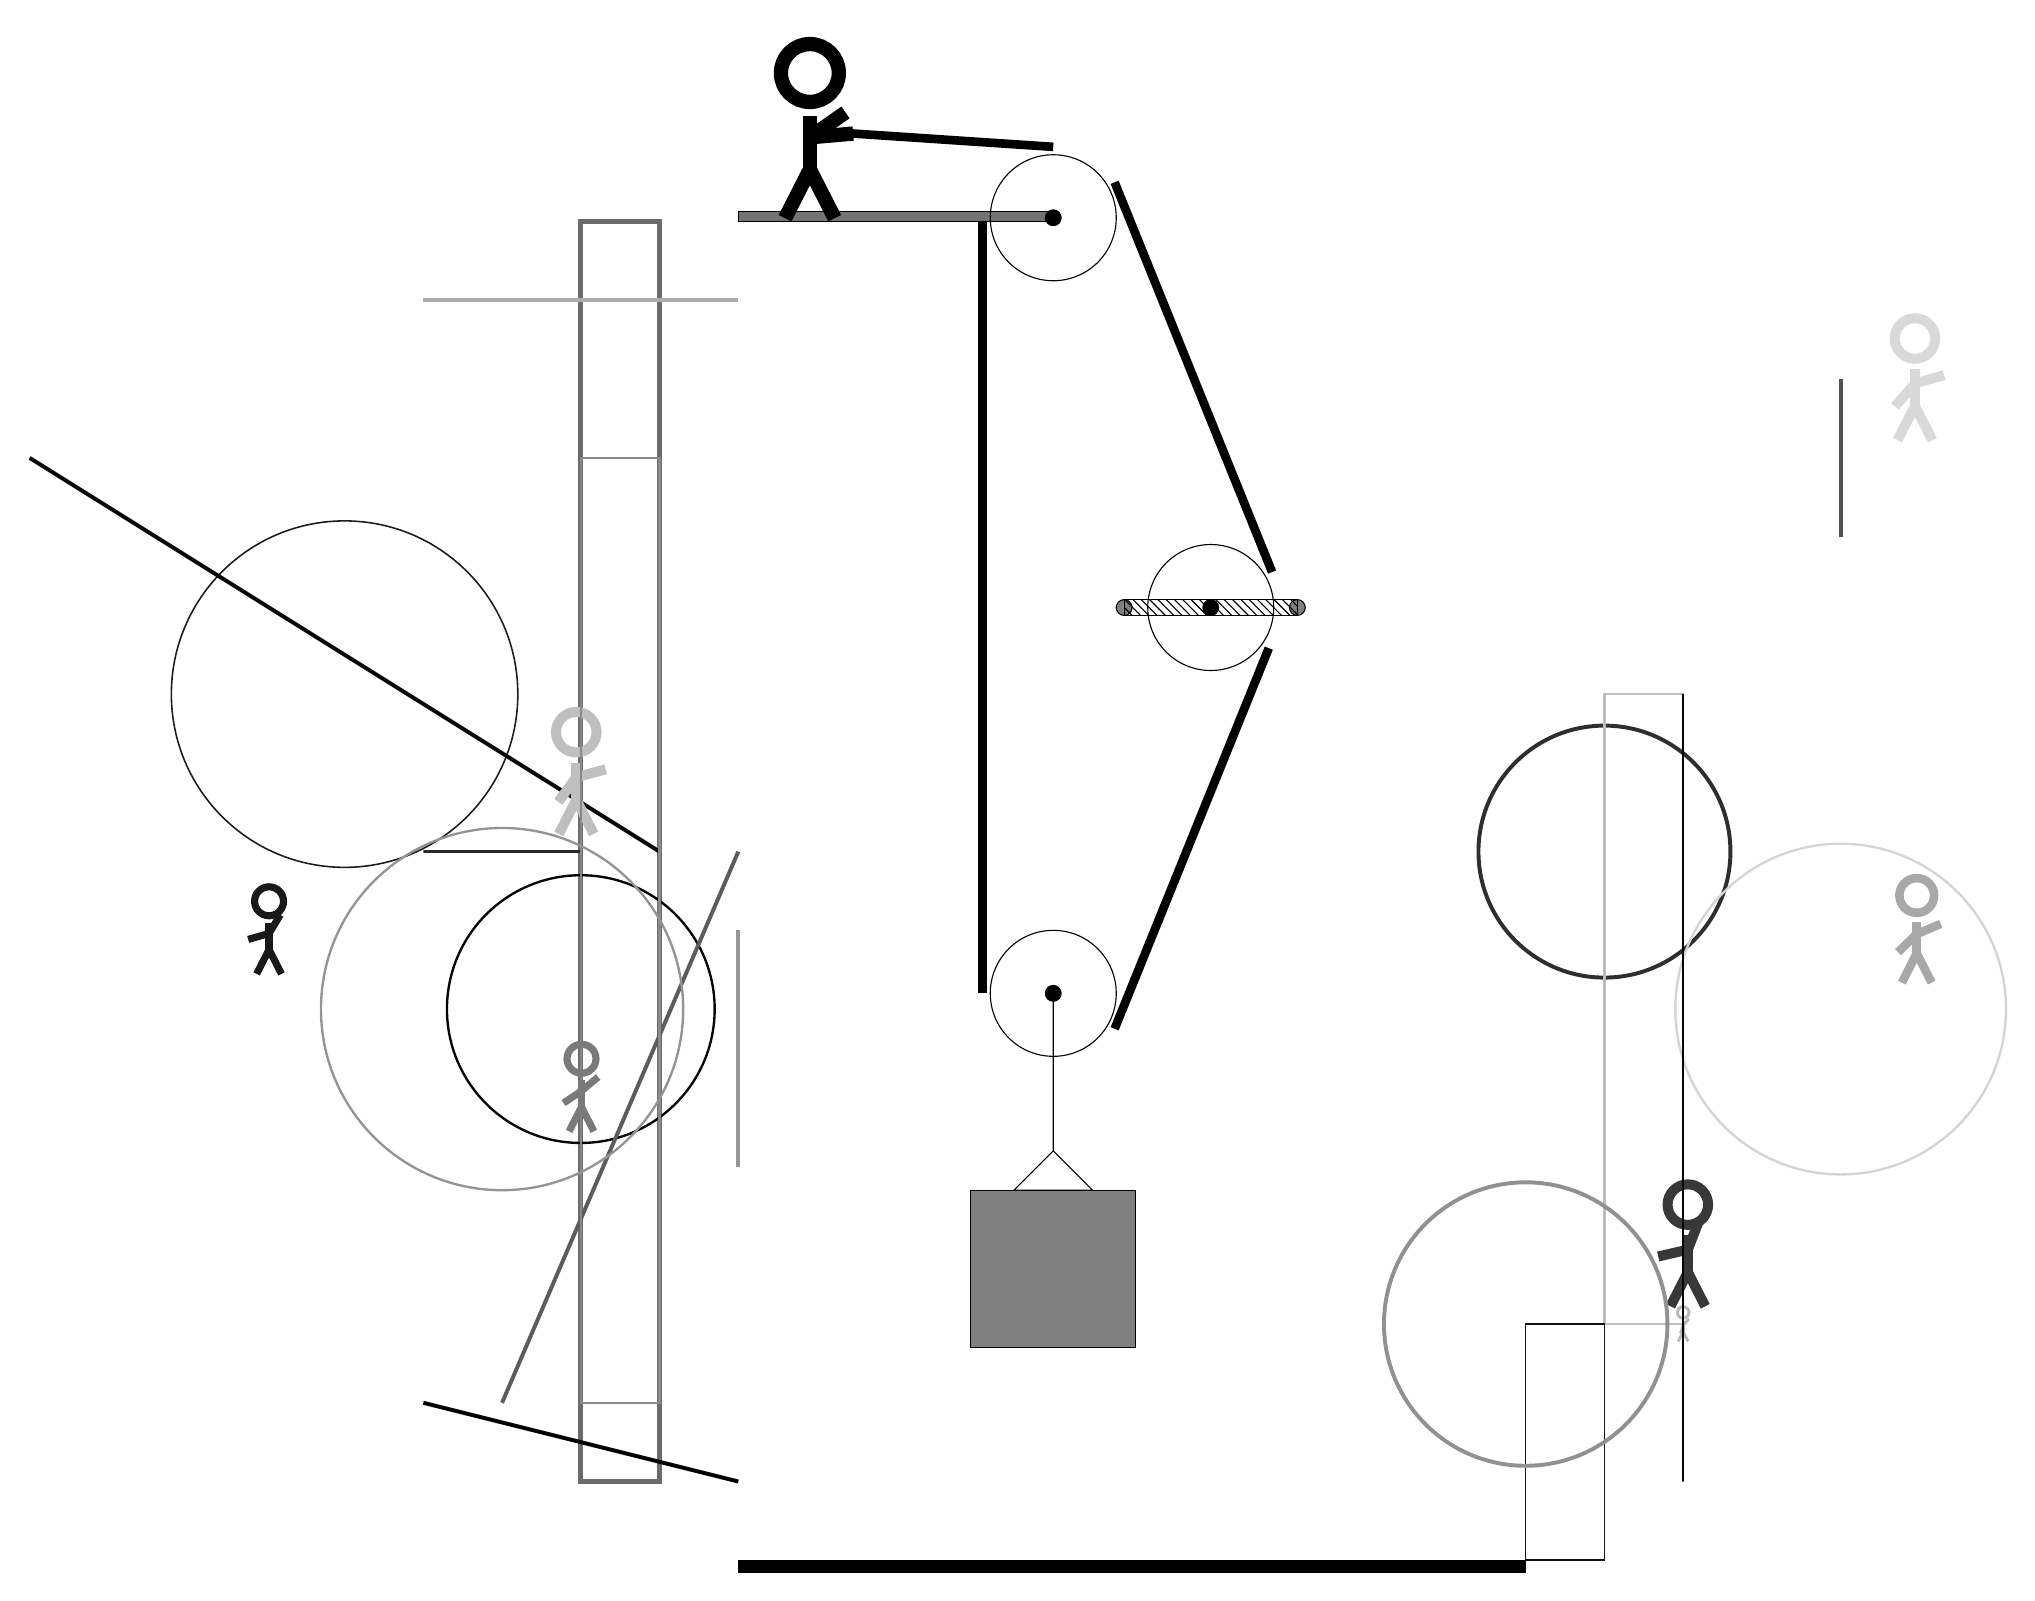
\begin{tikzpicture}
			%%%%% START %%%%%
			
			\draw[fill=black!55] (-2, 14) rectangle (2, 14.125);
			
			\draw (2, 4.2) circle (0.8);
			\draw[fill=black] (2, 4.2) circle (0.1);
			
			\draw (2, 14.05) circle (0.8);
			\draw[fill=black] (2, 14.05) circle (0.1);
			
			\draw[fill=white](4, 9.1) circle (0.8);
			\draw[fill=black] (4, 9.1) circle (0.1);
			\draw[fill=black!50] (2.9, 9.1) circle (0.1);
			\draw[fill=black!50] (5.1, 9.1) circle (0.1);
			\draw[pattern=north west lines, pattern color=black] (2.9, 9.2) rectangle (5.1, 9.0);
			
			\draw (2, 4.2) -- (2, 2.2) -- (1.5, 1.7) -- (2.5, 1.7) -- (2, 2.2);
			\draw[fill=black!50] (0.95, 1.7) rectangle (3.05, -0.3);
			
			\draw [line width=0.5mm, color=black!82](9, 6) circle (1.6);
			
			\draw[line width=0.6mm, color=black!58] (-4, -2) rectangle (-3, 14);
			\draw[line width=0.3mm, color=black!26] (9, 8) rectangle (10, 0);
			\draw[line width=0.5mm, color=black!33](-2, 13) -- (-6, 13);
			
			\draw [line width=0.2mm, color=black!89](-7, 8) circle (2.2);
			
			\node[line width=0.6mm, color=black!34] at (13, 5) {\Strichmaxerl[6][44][23]};
			\draw[line width=0.5mm, color=black!41](-2, 2) -- (-2, 5);
			
			\draw[line width=0.4mm, color=black!84] (-4, 6) rectangle (-6, 6);
			\draw [line width=0.3mm, color=black!17](12, 4) circle (2.1);
			
			\node[line width=0.5mm, color=black!78] at (10, 1) {\Strichmaxerl[7][13][69]};
			\draw [line width=0.3mm, color=black!98](-4, 4) circle (1.7);
			\node[line width=0.3mm, color=black!90] at (-8, 5) {\Strichmaxerl[5][16][59]};
			\node[line width=0.3mm, color=black!28] at (10, 0) {\Strichmaxerl[2][72][48]};
			
			\draw[line width=0.5mm, color=black!64](-5, -1) -- (-2, 6);
			\draw[line width=0.2mm, color=black!93] (9, -3) rectangle (8, 0);
			\draw[line width=0.5mm, color=black!97](-3, 6) -- (-11, 11);
			
			\node[line width=0.2mm, color=black!25] at (-4, 7) {\Strichmaxerl[7][54][15]};
			\draw [line width=0.5mm, color=black!43](8, 0) circle (1.8);
			\draw[line width=0.3mm, color=black!46] (-3, 11) rectangle (-4, -1);
			
			\draw[line width=0.5mm, color=black!99](-2, -2) -- (-6, -1);
			\node[line width=0.2mm, color=black!15] at (13, 12) {\Strichmaxerl[7][49][16]};
			\draw[line width=0.5mm, color=black!68](12, 10) -- (12, 12);
			
			\draw [line width=0.3mm, color=black!42](-5, 4) circle (2.3);
			\draw[line width=0.3mm, color=black!98] (10, 8) rectangle (10, -2);
			\node[line width=0.2mm, color=black!52] at (-4, 3) {\Strichmaxerl[5][34][40]};
			
			
			\draw[line width=1.1mm] (1.1, 14) -- (1.1, 4.2);
			\centerarc[line width=1.1mm](2, 4.2)(180:330:0.9);
			\draw[line width=1.1mm](2.7794, 3.75) -- (4.7373, 8.5838);
			\centerarc[line width=1.1mm](4, 9.1)(390:325:0.9);
			\draw[line width=1.1mm](4.7794, 9.55) -- (2.7794, 14.5);
			\centerarc[line width=1.1mm](2, 14.05)(30:90:0.9);
			\draw[line width=1.1mm](2, 14.95) -- (-1, 15.15);
			
			\node at (-1, 15.15) {\Strichmaxerl[10][-175][35]};
			
			\draw[fill=black] (-2, -3) rectangle (8, -3.15);
			
			%%%%% END %%%%%
		\end{tikzpicture}
	\end{figure}	
\end{document}